%EKG-7 Realisierung/Gehäuse
\subsection{Gehäuse}
Dieses Unterkapitel behandelt die Konstruktion des Gehäuses für das gesamte EKG Projekt. Zur Modellierung der 3D-Druck Teile wurde die Open Source Software Blender verwendet. Die Elektronik Komponenten sind dabei als externe STEP-Dateien importiert und im Gehäuse an der exakten Position platziert worden. \\
Das Display ist mit vier Stahl-Stützen über der Platine befestigt und ermöglicht so ein besonders kompaktes Design (Abbildung \ref{case_no_display1}). Das Langloch zum Tauschen der SD-Karte wird im gefertigte Zustand durch eine Gummi-Membran ausgefüllt und schützt so die Innere Elektronik vor Spritzwasser und Staub. Die folgenden gerenderten Bilder geben einen Einblick in das Konzept und Design der Box (Abbildung \ref{case_no_display1} und \ref{case_no_display2}) sowie des Deckels (Abbildung \ref{case_closed}).

\begin{figure} [!h]
	%\centering
	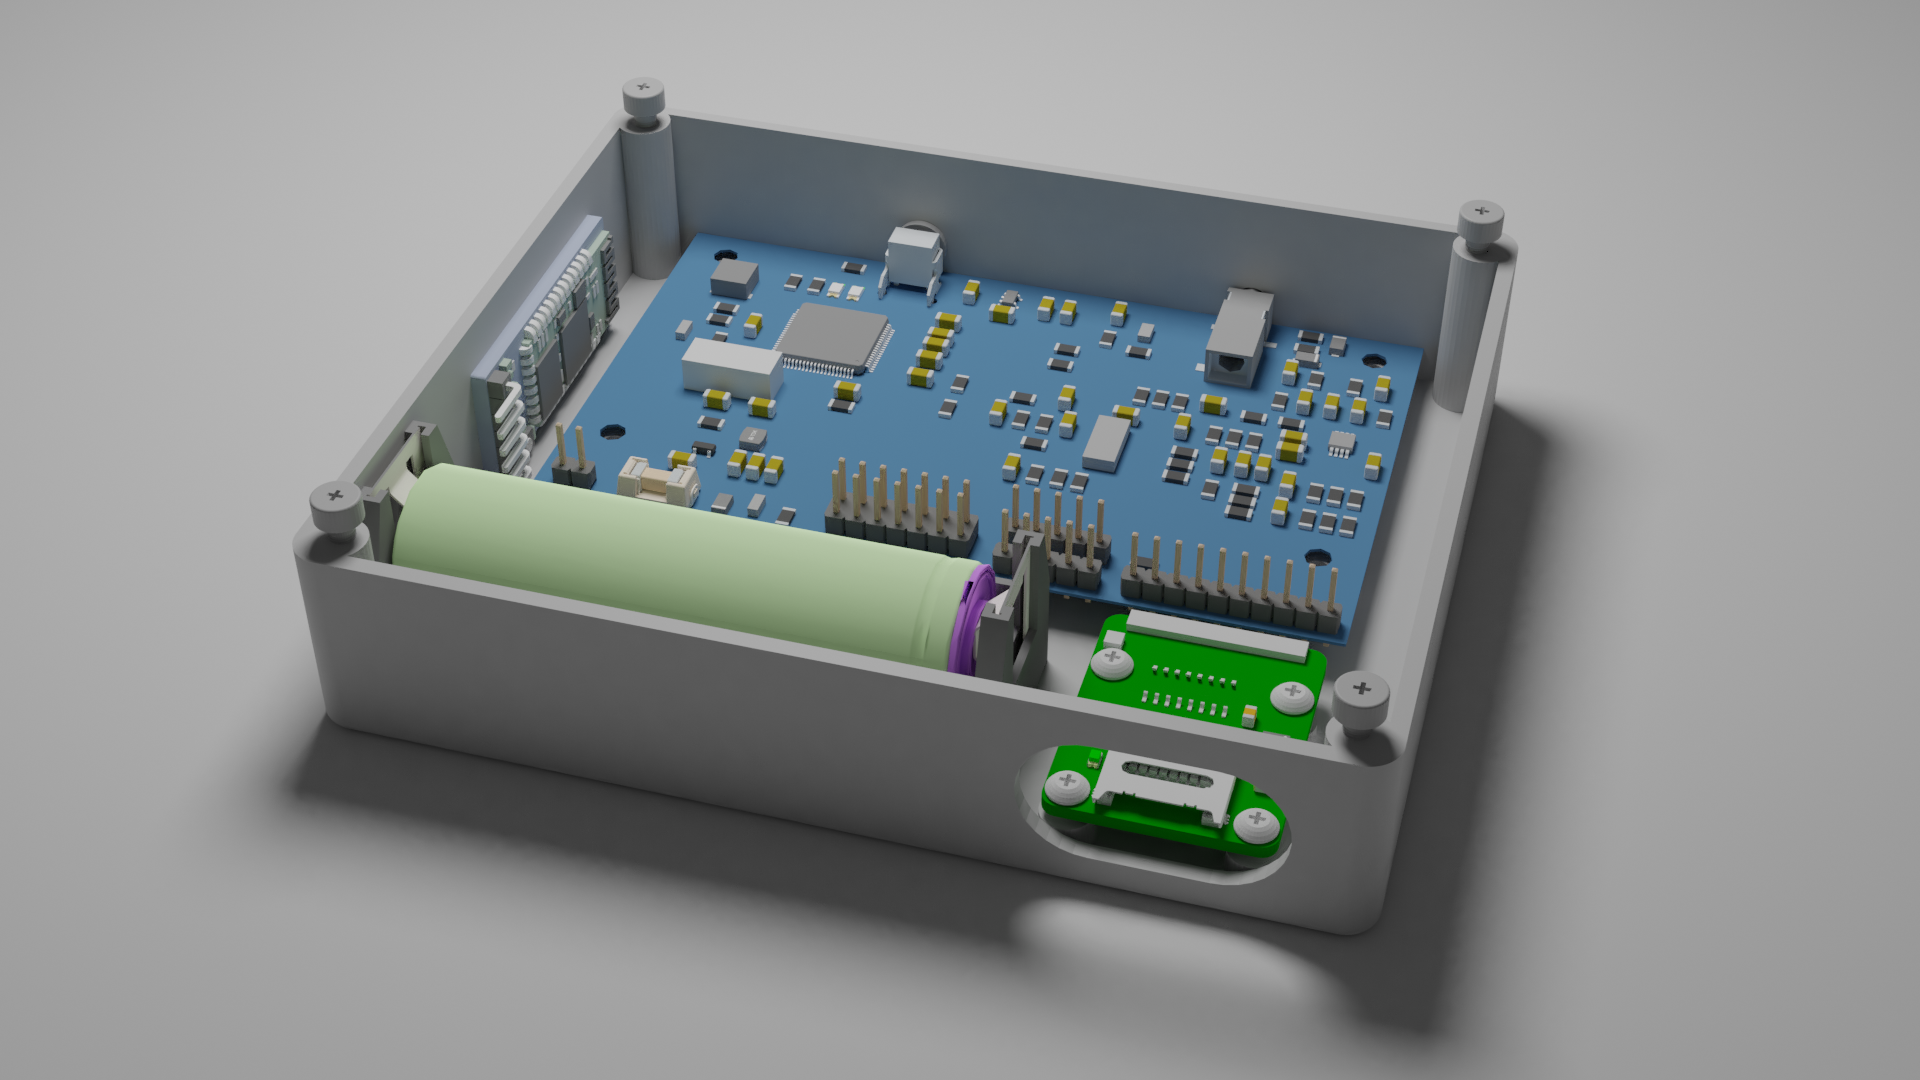
\includegraphics[width=\textwidth] {case_no_display.png}
	\caption{Vorderseite Gehäuse ohne Display}
	\label{case_no_display1} 
\end{figure}



\begin{figure} [!h]
	%\centering
	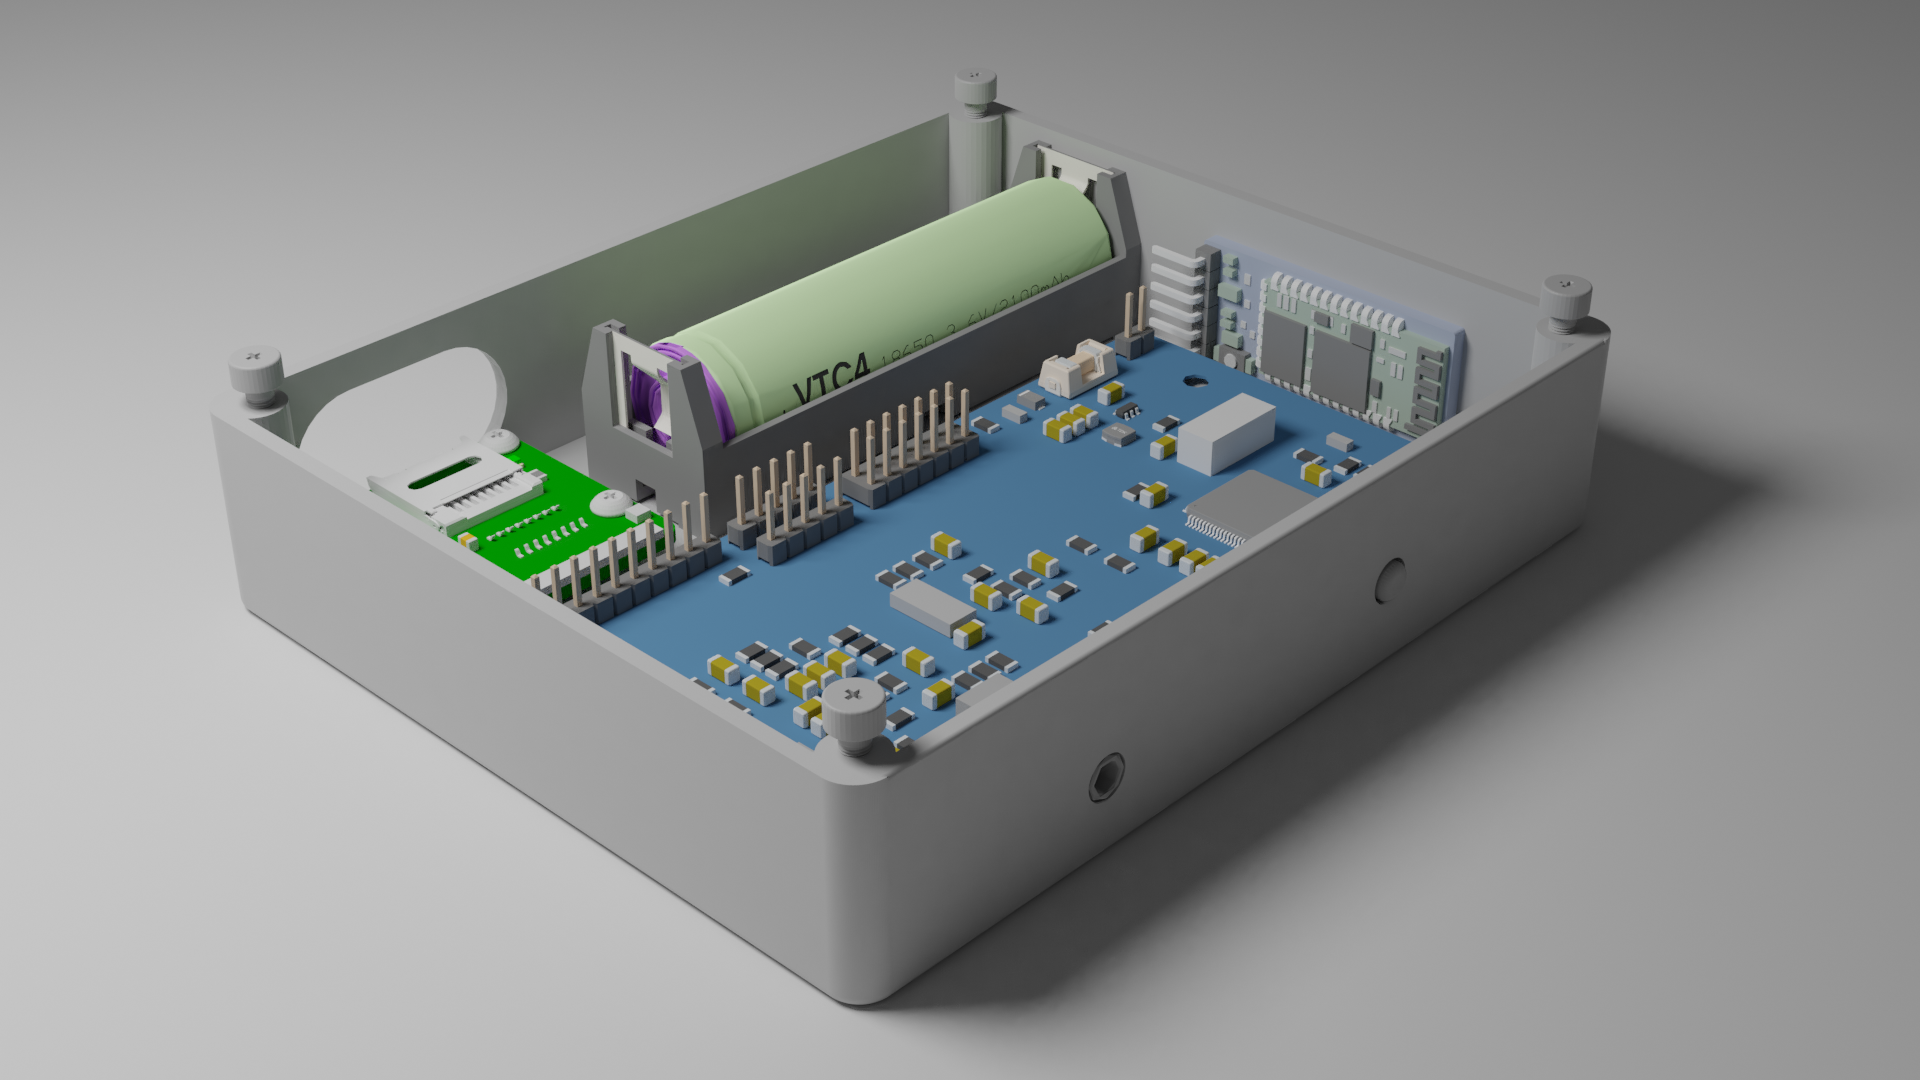
\includegraphics[width=\textwidth] {case_no_display_2.png}
	\caption{Rückseite Gehäuse ohne Display}
	\label{case_no_display2} 
\end{figure}

\begin{figure} [!h]
	%\centering
	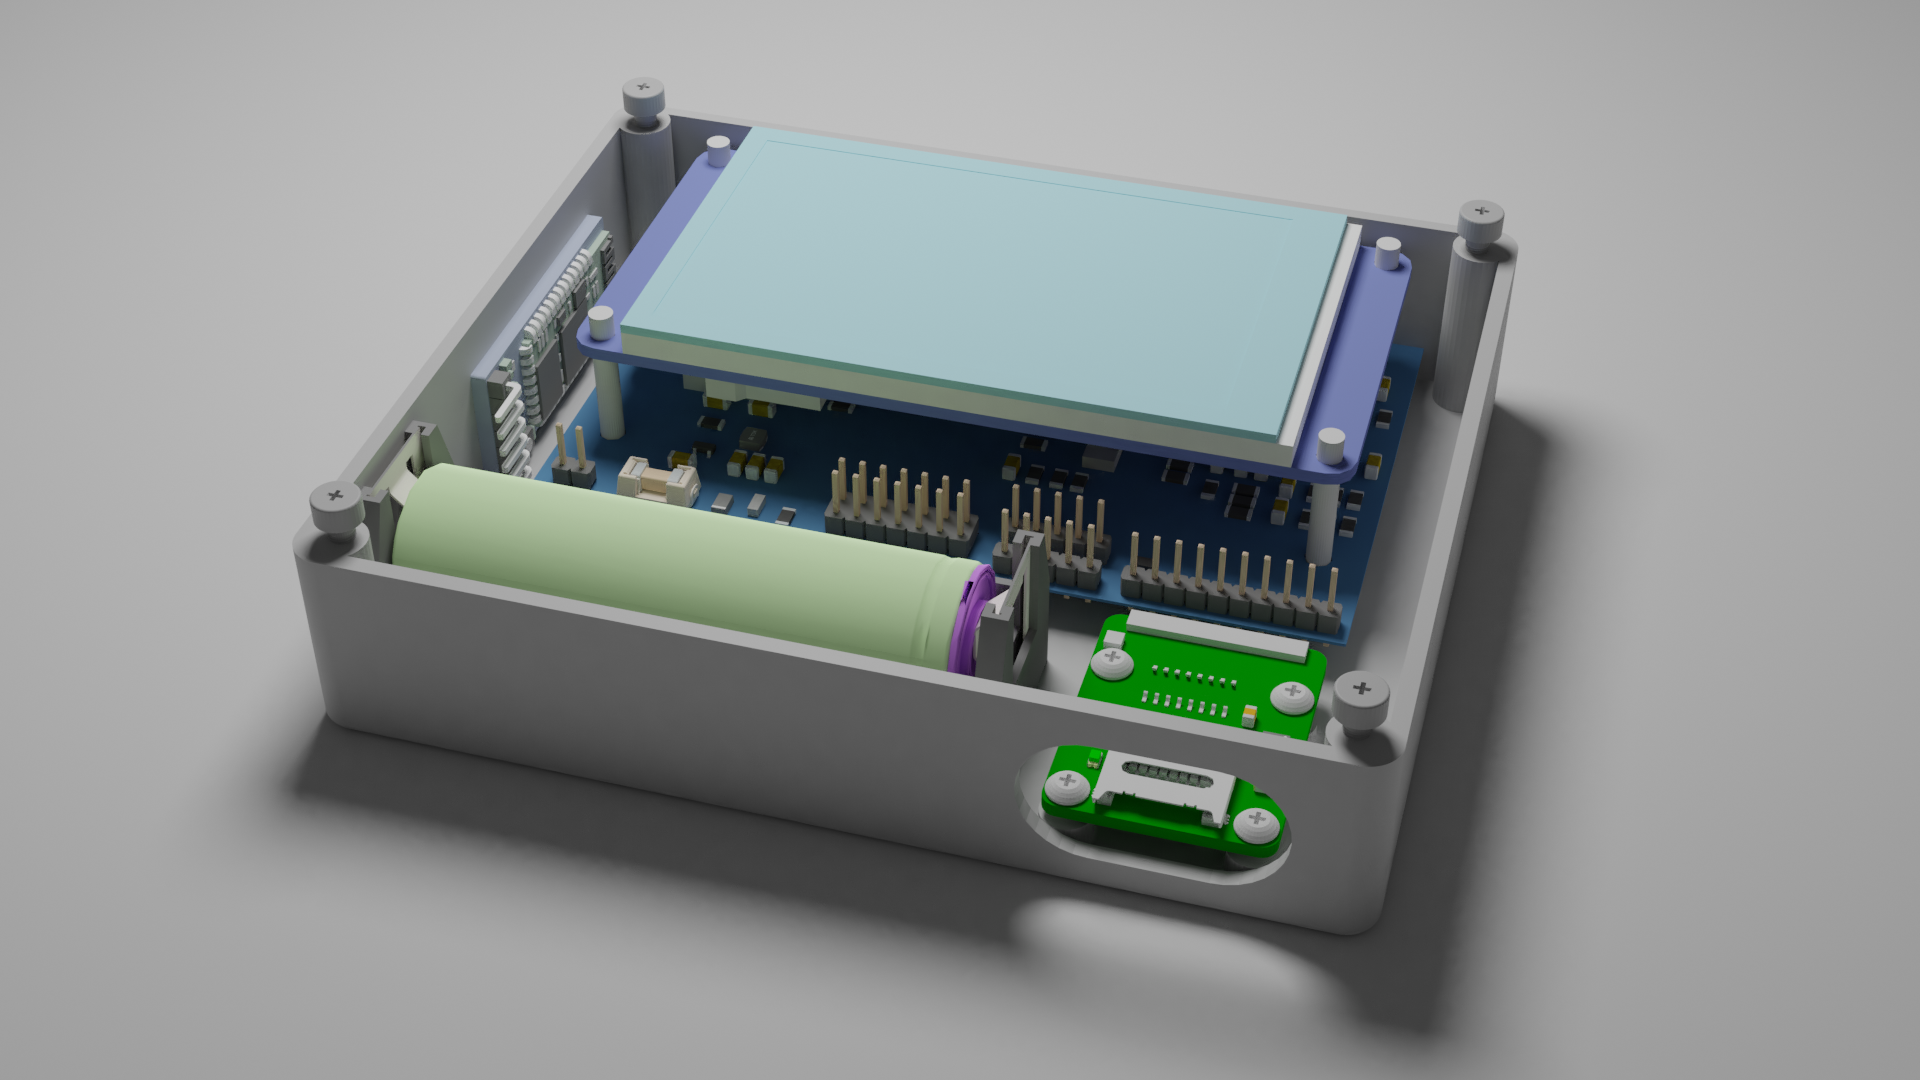
\includegraphics[width=\textwidth] {case_display.png}
	\caption{Gehäuse mit Display}
	\label{case_display} 
\end{figure}

\begin{figure} [!h]
	%\centering
	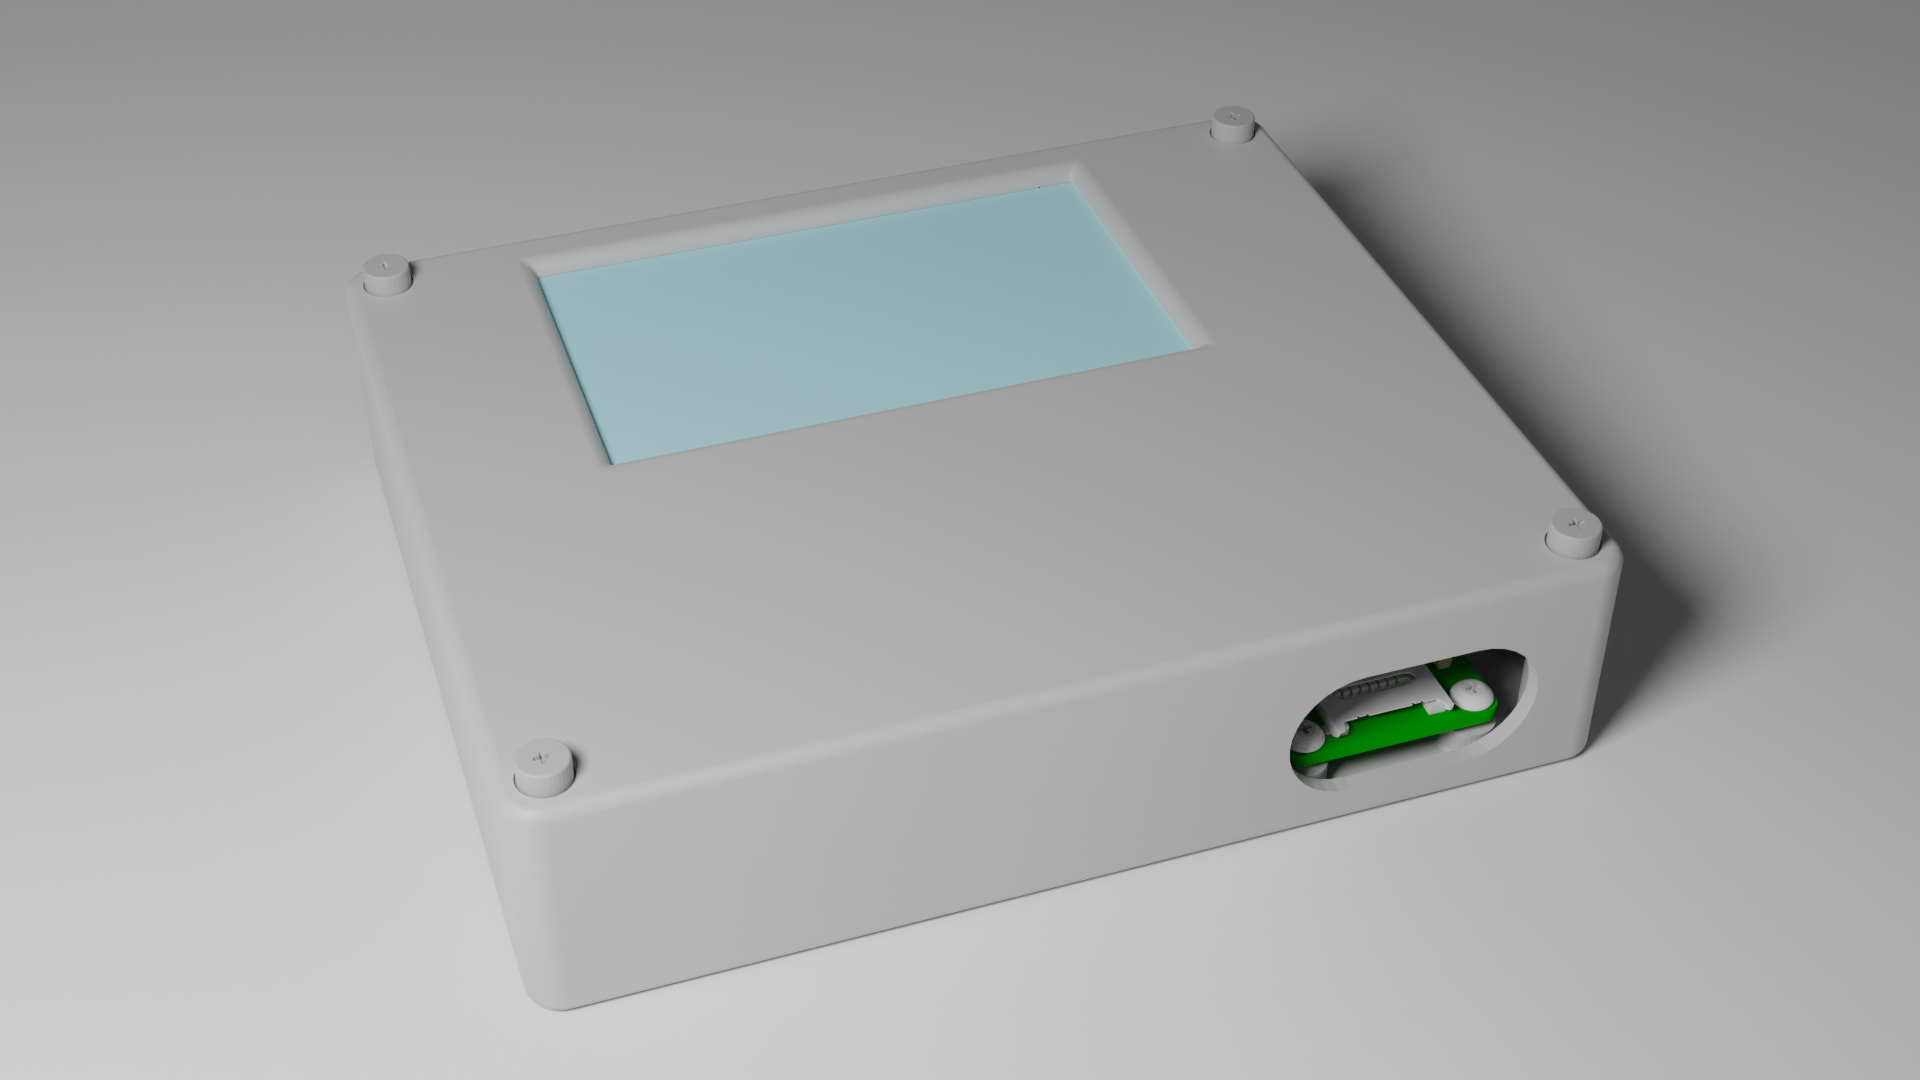
\includegraphics[width=\textwidth] {case_closed.png}
	\caption{Geschlossenes Gehäuse}
	\label{case_closed} 
\end{figure}

Um die Bedienung des Ein/Aus-Schalters zu vereinfachen wurde ein abgesetzter Zylinder konstruiert, der zwischen Platine und Gehäuse geklemmt wird.
\clearpage



